\documentclass[twocolumn,letterpaper,10pt]{article} 
\title{Project 3}
\hyphenpenalty=5000
\usepackage{graphicx}
\usepackage[dvips,letterpaper,nohead,nofoot]{geometry} 
\usepackage{amsmath}
\usepackage{nccmath}
\usepackage{multicol}
\usepackage{listings}
\usepackage{fancyvrb}

 \begin{document}

\twocolumn[%
\begin{center}
\textbf{ECE6100 Project 3}\\
Gavin Gresham\\
\rule{3in}{1pt}\\
\end{center}
] 

\section{Approach}
My approach was to use the program's main loop to parse the trace files and pass the instructions to various methods and data structures to keep track of the algorithm's state. During each iteration of this loop a cycle is first simulated and the next command in the file is then read and parsed. A method is then called to add the appropriate reservation station. If none are open, the method stalls until one is free.

During each loop a simple method is run to advance the algorithm and check for completed reservation stations. The cycle entry of each station is first decremented by one and then checked to see if the cycle is 0. If it is, the station tag is added to a queue. 

Once each reservation station has been checked, the first element of the queue is popped and that station is cleared, and the reservation station and register file are updated.

Psuedo code is included on the final page for a more detailed look at my implementation.

\section{Running the Code}
\subsection{Compiling}
\verb~g++ Project3.cpp -o Proj3~
\subsection{Executing}
\verb~./Proj3 <Trace> <Adder RS Size>~ \verb~<Multiplier RS Size> <Load Store Size>~

\bigskip
All of the command line arguments are required.

\section{Testing Strategy}
The goal of my testing was to ensure that the algorithm behaved correctly and meet all the criteria of the project. I used examples from class slides as known solutions that I could test against, and created other examples to test various hazards and faults. Following are the basic examples I used for hazards.

\bigskip
\textbf{RAW:}
\begin{Verbatim}[frame=single]
ADDD F2 F0 F4
ADDD F7 F0 F2
\end{Verbatim}

\bigskip
\textbf{WAR:}
\begin{Verbatim}[frame=single]
MULD F4 F0 F7
MULD F0 F4 F2
ADDD F2 F2 F7
\end{Verbatim}

\bigskip
\textbf{WAW:}
\begin{Verbatim}[frame=single]
MULD F4 F0 F7
ADDD F2 F0 F4
ADDD F4 F0 F7
\end{Verbatim}

After modifying the cycles of the various instructions to the values specified in class, I was able to see that my implementation was executing the instructions as expected. Once these simple cases were done, I began to test stalls that could occur in the system.

\bigskip
\textbf{CDB Contention:}
\begin{Verbatim}[frame=single]
MULD F0 F0 F0
LD F2 X
\end{Verbatim}

As these instructions complete during the same clock cycle, only one should be able to acquire the CDB. A stall was detected and the load was delayed until the next cycle.

\bigskip
\textbf{Reservation Station Contention:}
\begin{Verbatim}[frame=single]
MULD F0 F0 F0
MULD F1 F1 F0
MULD F2 F2 F0
MULD F3 F3 F0
\end{Verbatim}

Using these instructions I set the multiplier function unit to have 3 reservation stations. Upon trying to add the last instruction, a stall was detected and the simulation continued to execute cycles until a free space was open.

Additionally, I tested my implementation with the given trace file to ensure that larger examples would function correctly and to make sure my command line inputs were working as I intended. I believe these cases cover the data hazards and structural hazards that are needed for this project. These cases show that my code works for the general cases of these problems, and I can think of no edge cases that would break my implementation.

\section{Results}

\begin{figure}[bht]
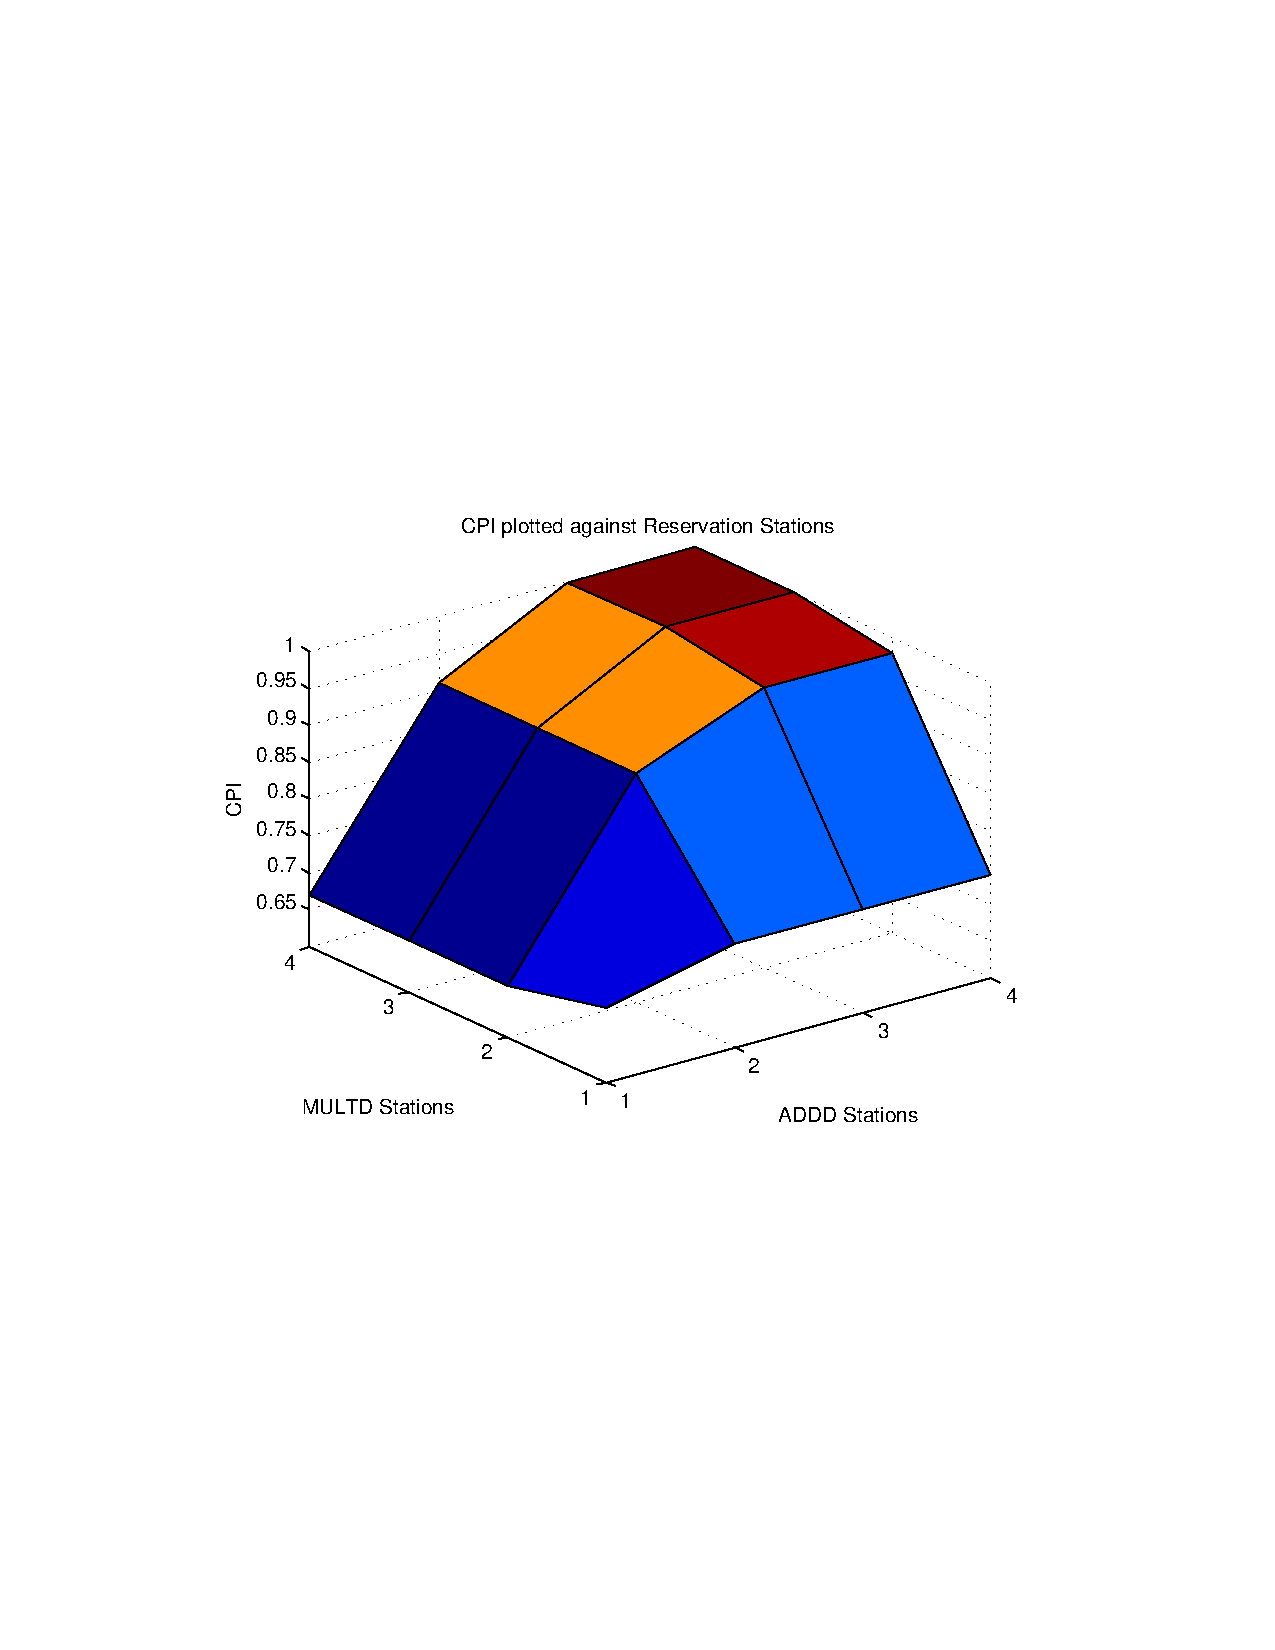
\includegraphics[scale=.5, clip=true, viewport=100 230 500 550]{CPI.pdf}
\caption{Performance of a given trace as a function of reservation stations.}
\label{fig:plot1}
\end{figure}

%\begin{figure}[bht]
%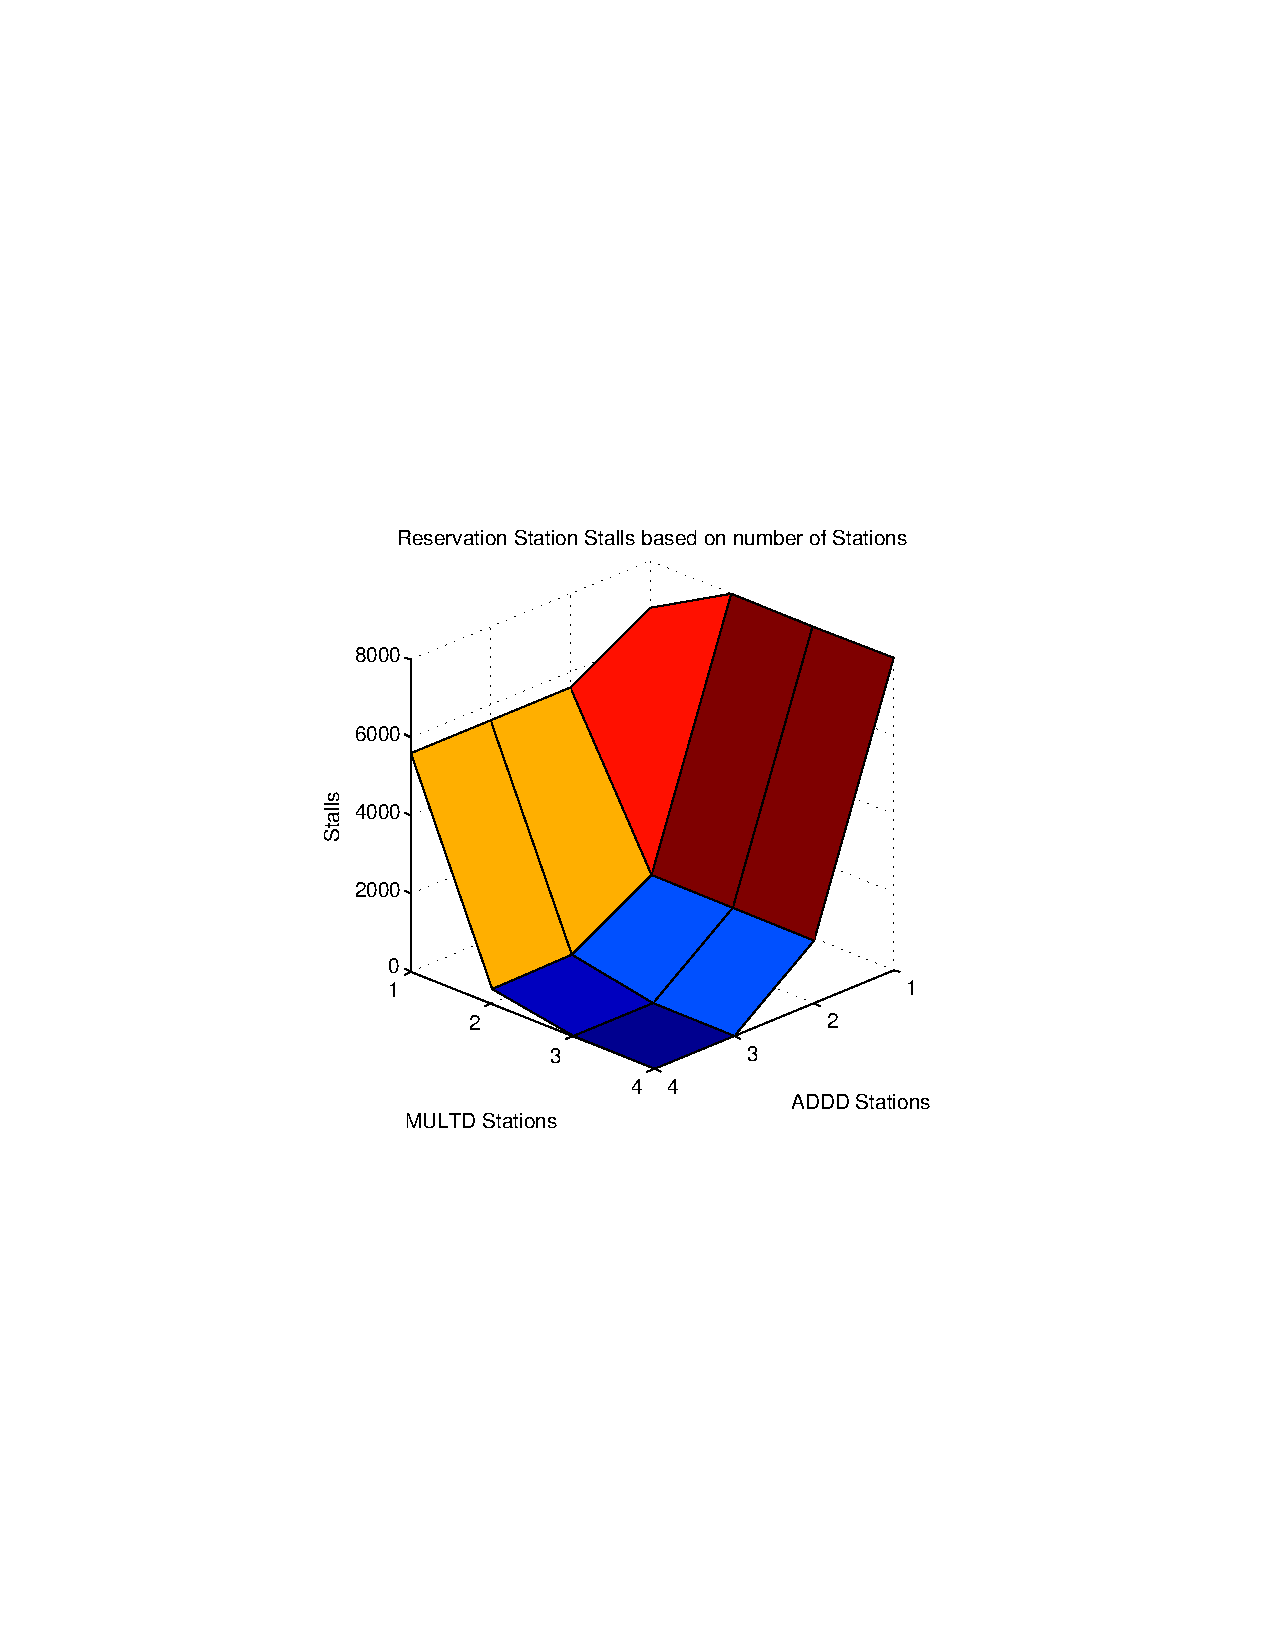
\includegraphics[scale=.5, clip=true, viewport=100 200 500 600]{RSStalls.pdf}
%\caption{}
%\label{fig:plot2}
%\end{figure}

%\begin{table}[bht]
%\begin{tabular}{|c|c|c|}
%\hline
%RS & CPI & RS Stalls\\
%1 & 0.68 & 7602\\\hline
%2 & .91 & 1600\\\hline
%3 & .91 & 1600\\\hline
%4 & .91 & 1600\\\hline
%\end{tabular}
%\caption{}
%\label{tbl:table1}
%\end{table}

Figure \ref{fig:plot1} shows the results of CPI based on number of reservation stations. While clearly more stations is better, there is a point of diminishing returns that needs to be considered. Adding extra components into a processor needs to be weighed against how much performance is gained.

With any functional unit having a single reservation station, there are significant performance impacts. Each instruction must wait until the previous one has finished executing, even if it was stalled and waiting for a dependency. A single reservation station is no better than a naive approach to scheduling, as no benefit is gained.

CPI and reservation station stalls appear to be inversely related from the data I gathered. As the number of stalls rises the CPI falls. This makes sense of course, as these stalls are lost potential that could be used to process additional instructions. Stalls waiting to aqcuire the commond data bus seem to be mostly unrelated to CPI however. There is little that can be done to ensure that multiple instructions don't complete at the same time, and any number of reservation stations over one runs the risk of experiencing a common data bus stall.

The importance slots for each functional unit seems to be about equal, with the adder increases the CPI at a slightly higher rate. If I were designing a dynamic scheduling component, I would elect to go with an even allocation of reservation stations. If the cost for adding another station was low enough, four for each the adder and the multiplier give the highest performance. Otherwise 3 adders and 2 or 3 multipliers give performance above 0.9 CPI and would be a good alternative. 

The minimal number of reservation stations I would prefer to use would be 3 adder stations and 2 multiplier stations. This seems to be the fewest number of reservation stations before any significant decrease in performance is seen.

\clearpage

\begin{lstlisting}[]
Main:
	For each Line in InputFile:
		ExecuteCycle()
		(Dest, Src1, Src2) = ParseInstruction(Line)
		AddToReservationStation(Dest, Src1, Src2)
	While ReservationStation not Empty:
		ExecuteCycle()

AddToReservationStation(Dest, Src1, Src):
	While no open in ReservationStation:
		ExecuteCycle()
	Station = first open in ReservationStation
	Station.Cycles = Instruction's Cycles

	Mark Dest as busy in the RegisterFile and set the Tag to Station

	If Src1 or Src2 are marked busy in RegisterFile:
		Set Station's tags to match the RegisterFile

ExecuteCycle()
	For each Station in ReservationStation:
		Decrement Station.Cycles
		If Station.Cycles == 0:
			Add Station to CompletionQueue
	
	If CompletionQueue not Empty:
		Station = CompletionQueue.Pop()
		Mark RegisterFile associated with Station.Dest not busy
		Clear this Station's Tag from other ReservationStations
		
\end{lstlisting}

\end{document}
